\section{Precision, feedback, and continual adaptation}
\label{sec:adaptation}

\subsection{Native precision and exact lattice replay}

The Phase~1 experiments met the reversibility and energy criteria.
After \PoneNeuralSteps{} steps on the neural tape, the absolute
\(L_2\) reconstruction errors in binary64 were \PoneNeuralQ{}
for position and \PoneNeuralP{} for momentum. In the double well,
the physical and shadow energy spans scaled as predicted over
the tested step sizes. Together, these results establish the
finite-horizon accuracy of the native implementation.

On the Phase~2 binary32 grid, both backends met the tolerance
through \PtwoGridLast{} steps and first missed it at
\PtwoGridFail{}. A separate scan of intervening prefixes
located the first absolute-error miss at \PtwoDenseCPU{} steps
on CPU and \PtwoDenseCUDA{} on CUDA, using the tolerance
\PtwoPrecisionThreshold{}. Neither first miss changed the
recovered first-task correct count. The int64 lattice state
returned bit for bit at every registered grid point through
\PtwoIntegerLast{} steps. This right-censored result comes with
two changes to the method: the lattice state occupies more
bytes than the binary32 phase state, and rounding changes the
forward update. Figure~\ref{fig:precision} shows absolute MLP
errors and relative Transformer errors in separate panels.

\begin{figure}[tbp]
  \centering
  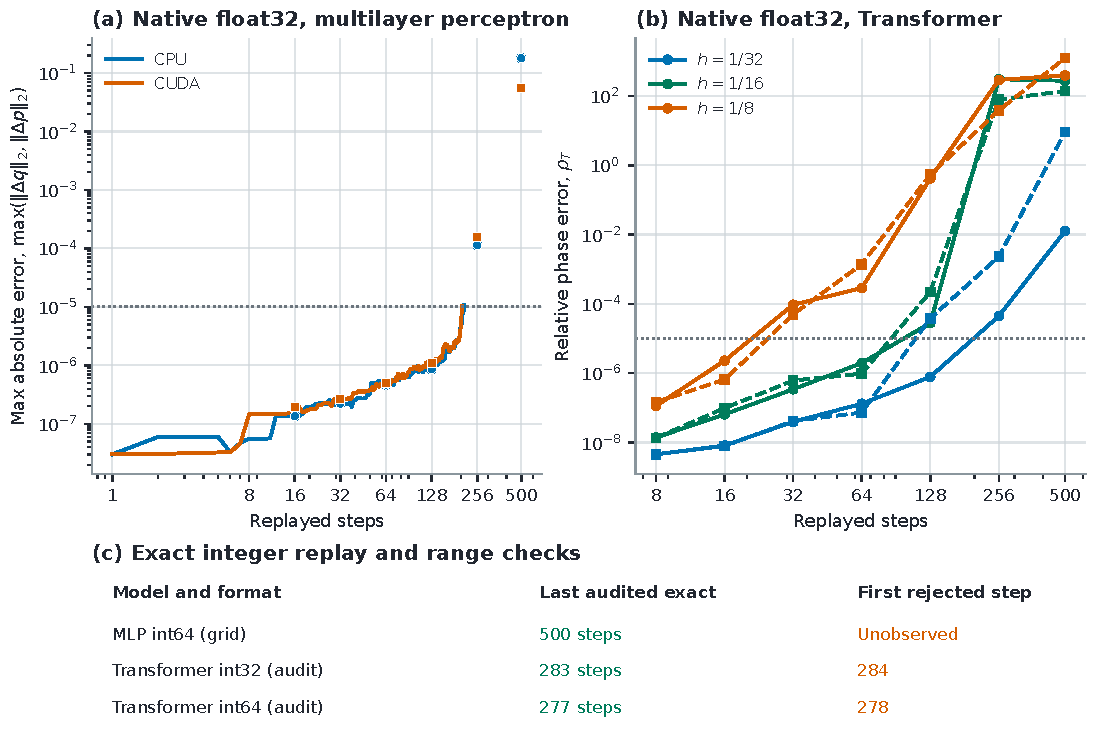
\includegraphics[width=\linewidth]{figures/fig1_precision_horizon.pdf}
  \caption{Measured replay precision on the MLP and Transformer.
  The panels use different error definitions. Native MLP curves
  use absolute component error, while Transformer curves use
  relative phase error. MLP lines show dense prefix measurements and
  markers show frozen-grid maxima across seeds. Transformer circles and
  squares identify the two seeds. Dotted guides mark the corresponding
  tolerances. Dense prefixes localize the MLP's first
  observed miss. Exact integer prefixes and range rejections
  identify tested endpoints of the long Transformer lattice runs.}
  \label{fig:precision}
\end{figure}

\begin{table}[tbp]
  \centering\small
  \caption{Phase~1 numerical and learning results from the
  confirmatory replication. The retention contrasts use the paired first-task
  backward-transfer margin.}
  \label{tab:phaseone}
  % Generated by scripts/build_tables.py
% Source: theory/evidence/phase1_replication_audit.json backends.cuda
% Source: artifacts/sol/analytic.json orders_physical_shadow
\begin{tabular}{@{}lr@{}}
\toprule
Outcome or paired contrast & CUDA result \\
\midrule
Neural f64 position L2 & \PoneNeuralQ \\
Neural f64 momentum L2 & \PoneNeuralP \\
Physical-energy orders & \ensuremath{2.0009,\;2.0007} \\
Shadow-energy orders & \ensuremath{4.0047,\;3.9997} \\
Glide poison detections & \PonePoisonsDetected/\PoneSeeds \\
Glide clean-window alarms & \PoneCleanAlarms/\PoneSeeds \\
AdamW-continue follow-up gap (pp) & \PoneAdamGap \\
\midrule
Fisher minus momentum SGD (pp; $p$) & \PoneFisherSGDDelta; \PonePrimaryP \\
Fisher minus AdamW (pp; $p$) & \PoneFisherAdamDelta; \PonePrimaryP \\
Fisher minus isotropic (pp; $p$) & \ensuremath{-3.000}; \ensuremath{1.000} \\
\bottomrule
\end{tabular}

\end{table}

\subsection{When feedback warrants rewind}

\paragraph{Phase~1.}
Glide detected \PonePoisonsDetected{}/\PoneSeeds{} poisoned windows
and raised \PoneCleanAlarms{} clean-window alarm, meeting the
pre-specified finite-horizon criterion. After \PoneFollowup{}
clean updates, AdamW under the continue-updating policy showed a
matched clean-minus-poison gap of \PoneAdamGap{} percentage points.
Because every poison alarm arrived before the first update, a
policy with the same signal and known boundaries could have
preserved its starting state by skipping a flagged window.
In the tested protocol, Glide committed the updates and rewound
at the window boundary. The observed accuracy advantage applies to
the comparison with continued adaptation. A matched pre-update
skip policy remains untested.

\paragraph{Phase~2 ramped onset (B2a).}
The delayed audit aggregates label disagreements within each block
of a stream with simulated annotation errors. A failed receipt authorizes
replay back to the start of the latest block, so an alarm that
arrives late can leave earlier corrupted updates outside the
replayable suffix. Glide recovered the intended origin in
\PtwoRampRecovered{}/\PtwoSeeds{} dirty windows, and B2a failed
the pre-specified pass criterion. In
\PtwoRampDamaged{}/\PtwoSeeds{} dirty windows, the rewind arm had
lost at least \PtwoDamageThreshold{} percentage points of
Task~1 accuracy at the alarm relative to the true-origin state.
The passive AdamW loss monitor signaled early in
\PtwoRampEarly{}/\PtwoSeeds{} windows. The tested onsets align
with the audit schedule.

\paragraph{Phase~2 terminal verifier (B2b).}
The updates use potentially corrupted teacher pseudo-labels, and
an independent first-task canary supplies one actionable bit at
the end of each window. Rewind recovered
\PtwoTerminalRecovered{}/\PtwoSeeds{} dirty origins within the
pre-specified phase error tolerance \PtwoAlarmTargetTol{}.
B2b met the pre-specified pass criterion. The Task~1 accuracy
drop met the same damage criterion at the alarm in
\PtwoTerminalDamaged{}/\PtwoSeeds{} dirty windows. Clean terminal alarms occurred in
\PtwoTerminalAdamSkipCleanAlarms{}/\PtwoSeeds{} windows for AdamW-skip
and \PtwoTerminalAdamContinueCleanAlarms{}/\PtwoSeeds{} for
AdamW-continue. By the terminal signal, AdamW has already
committed the \PtwoTerminalUpdates{} updates that an earlier
skip would have prevented. Compared with
\emph{terminal-only AdamW-skip}, rewind gained
\PtwoTerminalAdamImmediate{} percentage points immediately and
\PtwoTerminalAdamBudget{} points at the common
\PtwoTerminalBudget{}-gradient budget, which lets non-replay
policies spend their remaining gradients on clean repair.

\paragraph{Exploratory early-skip control.}
After examining the held-out outcomes, we tested whether
disagreement with a majority of the teacher pseudo-labels could
serve as a pre-update warning for AdamW. The policy froze its
weights and moments before the flagged update and used its
remaining gradient credits for clean repair. Monitoring required
an additional forward pass per batch, and we did not measure its
wall-time cost. The warning appeared after \PtwoEarlyWarnFirst{}
to \PtwoEarlyWarnLast{} commits in \PtwoEarlyWarnDirty{}/\PtwoSeeds{}
dirty windows and \PtwoEarlyWarnClean{}/\PtwoSeeds{} clean windows.
On the same seeds, early skip and rewind gave
\PtwoEarlySkipImmediateCorrect{} and \PtwoRewindImmediateCorrect{}
correct predictions out of \PtwoTerminalTotal{} at window end.
At equal gradient budget the counts were
\PtwoEarlySkipBudgetCorrect{} and \PtwoRewindBudgetCorrect{}.
Although rewind recovered within the pre-specified tolerance,
its accuracy advantages over early skip were only
\PtwoEarlyImmediateDelta{} and \PtwoEarlyBudgetDelta{} percentage
points on these tapes. A confirmatory comparison would require
fresh test seeds.

\begin{table}[tbp]
  \centering\small
  \caption{Phase~2 recovery under the pre-specified policies and
  the post-hoc early-skip control. Clean alarm counts are reported
  separately for each policy over \PtwoSeeds{} clean windows per regime.
  The damage count uses dirty DKD-rewind windows that
  lost at least \PtwoDamageThreshold{} percentage points of Task~1
  accuracy at alarm relative to the true-origin state.
  The terminal-only baseline acts after the full speculative window.}
  \label{tab:recovery}
  % Generated by scripts/build_tables.py
% Source: theory/evidence/phase2/sol_replication_audit.json backends.cuda.B and exploratory_B2b.effects.dirty
% Source: artifacts/sol/p2/sol-20261122-cpu-lock/test_cuda.json B[*].{a,b}.{dirty,clean}.policies
\begin{tabular}{@{}lrr@{}}
\toprule
Outcome & Ramped & Terminal \\
\midrule
True-origin recoveries & \ensuremath{9/12} & \PtwoTerminalRecovered/\PtwoSeeds \\
Dirty DKD rewind damage at alarm ($\geq\PtwoDamageThreshold$ pp) & \ensuremath{0/12} & \ensuremath{12/12} \\
Dirty DKD rewind alarms & \ensuremath{12/12} & \ensuremath{12/12} \\
Clean DKD rewind alarms & \ensuremath{0/12} & \ensuremath{0/12} \\
Clean AdamW-skip alarms & \ensuremath{0/12} & \ensuremath{4/12} \\
Clean AdamW-continue alarms & \ensuremath{0/12} & \ensuremath{4/12} \\
Rewind minus AdamW-skip, immediate (pp) & \ensuremath{0.78} & \PtwoTerminalAdamImmediate \\
Rewind minus AdamW-skip, equal budget (pp) & \ensuremath{-0.94} & \PtwoTerminalAdamBudget \\
Pre-specified verdict & Fail & Pass \\
\midrule
\multicolumn{3}{@{}l@{}}{\textit{Exploratory control on terminal dirty windows}} \\
Correct over \PtwoTerminalTotal & Immediate & Equal budget \\
Early-skip AdamW & \PtwoEarlySkipImmediateCorrect & \PtwoEarlySkipBudgetCorrect \\
DKD rewind & \PtwoRewindImmediateCorrect & \PtwoRewindBudgetCorrect \\
Rewind minus early skip (pp) & $+$\PtwoEarlyImmediateDelta & $+$\PtwoEarlyBudgetDelta \\
\bottomrule
\end{tabular}

\end{table}

\subsection{Fisher guidance fell short on retention}

The Phase~1 Fisher brake damps the low-Fisher momentum block.
Momentum in the high-Fisher block can still move the parameters
away from the old solution. At a common incoming state, the
projected brake also removes less kinetic energy than isotropic
damping when that high-Fisher block carries momentum, so the
isotropic comparison mixes orientation and strength. The Fisher
brake's mean Task~1 BWT contrasts against
momentum SGD and AdamW are \PoneFisherSGDDelta{} and
\PoneFisherAdamDelta{} percentage points, respectively. Both
one-sided tests give \(p=\PonePrimaryP{}\) at the registered
margin. For the Fisher arm, mean first-task accuracy falls from
\PoneFisherStartPct{}\% to \PoneFisherEndPct{}\%, while mean live
accuracy is \PoneFisherLivePct{}\%. The isotropic ablation also
has better observed retention than the projected brake.
These comparisons are for fixed settings
under an incoming-batch budget.

Phase~2 Fisher mass slows movement along high-Fisher coordinates
for a given momentum. The drift still has no anchor to the old
weights. Fisher mass met the live accuracy criterion and failed
each primary retention contrast. GENERIC adds that anchor and
cleared the absolute live accuracy floor, but it fell short
against tuned AdamW (\PtwoGenericLivePct{}\% versus
\PtwoAdamLivePct{}\%). Its BWT gain over the matched mass control
was \PtwoGenericMassDelta{} percentage points, with
\(p=\PtwoGenericMassP{}>\PtwoCutoff{}\). EWC supplies a conventional
restoring-force comparator under the same fresh gradient budget.
The damping arms matched realized energy removal by capping the
nominal request when a projected arm had insufficient kinetic
energy. The cap was active on \PtwoCaps{} of \PtwoEnergySteps{} steps,
precluding inference about orientation at the nominal isotropic
strength. The high-versus-low BWT contrast also failed its
superiority criterion. Figure~\ref{fig:retention} shows the paired
contrasts against the positive test margin. Equivalence remains
untested.

\begin{table}[tbp]
  \centering\small
  \caption{Confirmatory Phase~2 retention contrasts. Positive paired
  differences favor the named intervention. Sign tests use the
  pre-specified positive BWT margin and familywise cutoff.}
  \label{tab:retention}
  % Generated by scripts/build_tables.py
% Source: theory/evidence/phase2/sol_replication_audit.json backends.cuda.C.{mass,generic,high}.contrasts
\begin{tabular}{@{}llrrr@{}}
\toprule
Method & Comparator & $\Delta\mathrm{BWT}$ (pp) & Wins / non-ties & One-sided $p$ \\
\midrule
Fisher mass & Momentum SGD & \ensuremath{-14.67} & \ensuremath{0/12} & \ensuremath{1.000} \\
Fisher mass & AdamW & \ensuremath{-4.89} & \ensuremath{0/11} & \ensuremath{1.000} \\
Fisher mass & EWC & \ensuremath{-35.64} & \ensuremath{0/12} & \ensuremath{1.000} \\
Fisher mass & unit mass & \ensuremath{2.36} & \ensuremath{5/12} & \ensuremath{0.8062} \\
GENERIC & Momentum SGD & \ensuremath{-8.81} & \ensuremath{1/12} & \ensuremath{0.9998} \\
GENERIC & AdamW & \ensuremath{0.97} & \ensuremath{4/12} & \ensuremath{0.9270} \\
GENERIC & EWC & \ensuremath{-29.78} & \ensuremath{0/12} & \ensuremath{1.000} \\
GENERIC & Fisher mass & \ensuremath{5.86} & \ensuremath{9/11} & \ensuremath{0.0327} \\
High Fisher & low Fisher & \ensuremath{-0.75} & \ensuremath{0/12} & \ensuremath{1.000} \\
\bottomrule
\end{tabular}

\end{table}

\begin{figure}[tbp]
  \centering
  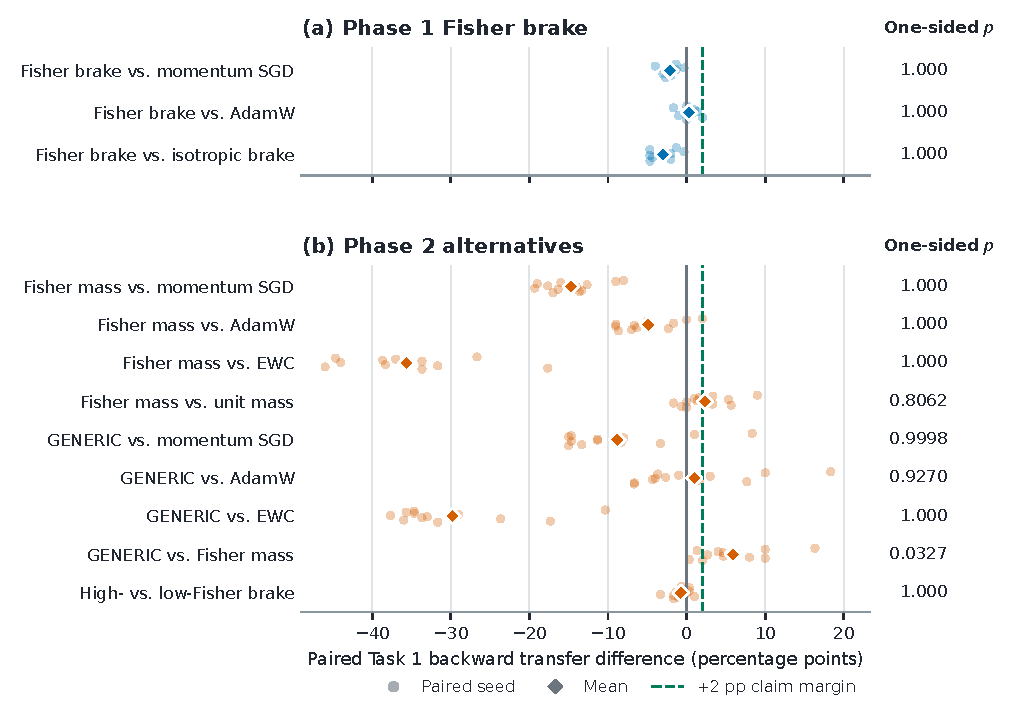
\includegraphics[width=\linewidth]{figures/fig2_continual_falsification.pdf}
  \caption{Paired backward-transfer contrasts in both continual
  phases. Marks show seed differences and their means. The
  registered tests compare with a positive superiority margin,
  so a positive mean alone does not pass.}
  \label{fig:retention}
\end{figure}
